%META {"question":"Tam giác ABC, D là điểm trên cạnh BC, nối A với D. Trên hình có tất cả bao nhiêu góc (không kể góc bẹt)?","options":["7 góc","5 góc","6 góc","8 góc"],"answer":0,"note":"Tại A có 3 góc (BAD, DAC, BAC); tại B và C mỗi nơi 1 góc; tại D có 2 góc (ADB, ADC). Tổng: 3 + 1 + 1 + 2 = 7 góc."}
\documentclass[border=5pt]{standalone}
\usepackage{tkz-euclide}
% Màu dùng chung cho toàn bộ hình vẽ (ảnh stack với nền tối của web)
\definecolor{tminc}{RGB}{226,232,240}   % chữ + nét chính
\definecolor{tmblue}{RGB}{0,210,255}    % nhấn neon xanh
\definecolor{tmpink}{RGB}{255,0,200}    % nhấn neon hồng
\definecolor{tmgreen}{RGB}{0,255,136}   % nhấn neon xanh lá
\color{tminc}

\begin{document}
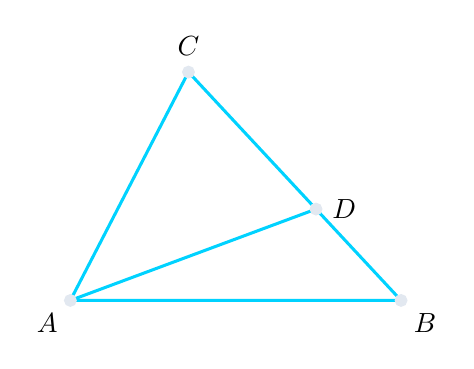
\begin{tikzpicture}[line width=1.1pt]
  \coordinate (A) at (0,0);
  \coordinate (B) at (4.2,0);
  \coordinate (C) at (1.5,2.9);
  \coordinate (D) at (3.12,1.16);
  \tkzDrawPolygon[tmblue,line width=1.1pt](A,B,C)
  \draw[tmblue] (A) -- (D);
  \tkzDrawPoints[size=3.5,color=tminc,fill=tminc](A,B,C,D)
  \tkzLabelPoint[below left=1pt](A){$A$}
  \tkzLabelPoint[below right=1pt](B){$B$}
  \tkzLabelPoint[above=2pt](C){$C$}
  \tkzLabelPoint[right=2pt](D){$D$}
\end{tikzpicture}
\end{document}
